\documentclass{clbeamer2024}

\usepackage{minted}

\usepackage{minted}
\setminted{
	breaklines=true,
	frame=single,
	bgcolor=lightgray,
	fontsize=\small,
	escapeinside=||
}

\usepackage{xcolor}
\definecolor{bg}{rgb}{0.95, 0.95, 0.92} % Couleur gris clair

\title{
	%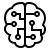
\includegraphics[width=0.5cm]{logos/IA1.png} \hfill
        Introduction à React
	
\includegraphics[width=0.7cm]{logos/react.png} \hfill
}
\subtitle{Comprendre les bases de la bibliothèque JavaScript pour les interfaces utilisateur}
\author{Slimani Mohamed Amine}
\institute{EHTP}
\date{\today}

\begin{document}
	\setcounter{framenumber}{-1}
	\frame{\titlepage}
	
	
	
	% Sommaire
	\begin{frame}{Sommaire}
		\tableofcontents
	\end{frame}
	
	
	\section{Qu'est-ce que React ?}
	\begin{frame}{Qu'est-ce que React ?}
		\begin{itemize}
			\item \textbf{Définition} : React est une bibliothèque JavaScript open-source développée par Facebook pour construire des interfaces utilisateur.
			\item \textbf{Objectif} : Permettre de créer des applications web interactives et performantes.
			\item \textbf{Avantages} : Composants réutilisables, DOM virtuel, et grande communauté.
		\end{itemize}
	\end{frame}
	
	\section{Pourquoi utiliser React ?}
	\begin{frame}{Pourquoi utiliser React ?}
		\begin{itemize}
			\item \textbf{Composants réutilisables} : Permet de créer des composants modulaires et réutilisables.
			\item \textbf{Performance} : Utilisation du DOM virtuel pour des mises à jour efficaces.
			\item \textbf{Écosystème riche} : De nombreuses bibliothèques et outils disponibles.
		\end{itemize}
	\end{frame}
	
	\section{Concepts de base de React}
	\begin{frame}{Concepts de base de React}
		\begin{itemize}
			\item \textbf{Composants} : Blocs de construction de base d'une application React.
			\item \textbf{JSX} : Syntaxe qui permet d'écrire du HTML dans JavaScript.
			\item \textbf{État (State)} : Données internes d'un composant qui peuvent changer.
			\item \textbf{Props} : Données passées d'un composant parent à un composant enfant.
		\end{itemize}
	\end{frame}
	
	\section{Exemple de composant React}
	\begin{frame}{Exemple de composant React}
		\begin{exampleblock}{Composant fonctionnel en React}
			\begin{figure}[h] % "h" pour placer les images ici
				\centering
				\begin{minipage}{0.45\textwidth}
					\centering
					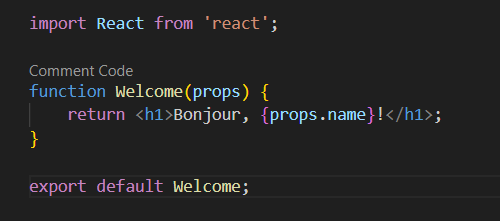
\includegraphics[width=\linewidth]{images/code1.png}
					%\caption{Code}
					\label{fig:image1}
				\end{minipage}
				\hfill % Espace flexible entre les images
				\begin{minipage}{0.38\textwidth}
					\centering
					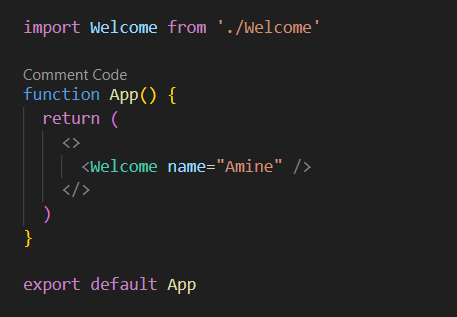
\includegraphics[width=\linewidth]{images/code2.png}
					%\caption{Résultat}
					\label{fig:image2}
				\end{minipage}
			\end{figure}
			\centering
			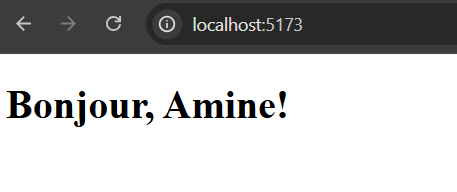
\includegraphics[width=0.7\textwidth]{images/resultat1.png}
		\end{exampleblock}
	\end{frame}
	
	
	\section{Gestion de l'état avec useState}
	\begin{frame}{Gestion de l'état avec useState}
		\begin{exampleblock}{Utilisation de useState pour gérer l'état}
			
			\begin{figure}[h] % "h" pour placer les images ici
				\centering
				\begin{minipage}{0.45\textwidth}
					\centering
					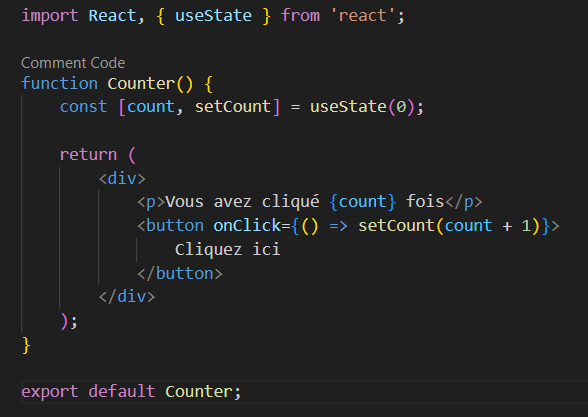
\includegraphics[width=\linewidth]{images/code3.png}
					%\caption{Code}
					\label{fig:image1}
				\end{minipage}
				\hfill % Espace flexible entre les images
				\begin{minipage}{0.4\textwidth}
					\centering
					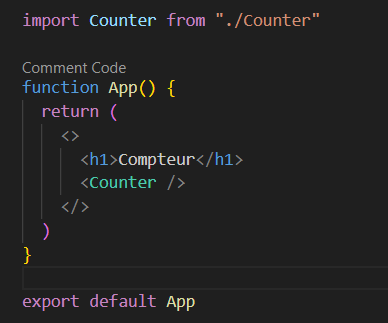
\includegraphics[width=\linewidth]{images/code4.png}
					%\caption{Résultat}
					\label{fig:image2}
				\end{minipage}
			\end{figure}
			\centering
			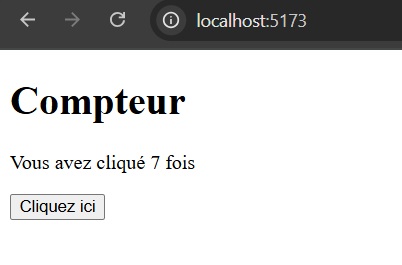
\includegraphics[width=0.4\textwidth]{images/resultat2.png}
		
		\end{exampleblock}
	\end{frame}
	
	\begin{frame}{Effets secondaires avec useEffect}
		\begin{exampleblock}{Utilisation de useEffect pour les effets secondaires}
			
			\begin{figure}[h] % "h" pour placer les images ici
				\centering
				\begin{minipage}{0.45\textwidth}
					\centering
					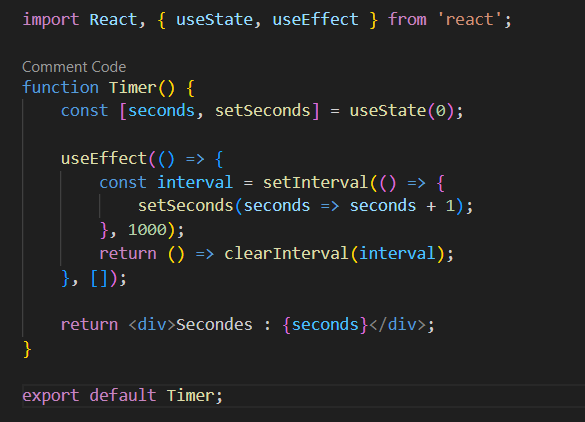
\includegraphics[width=\linewidth]{images/code5.png}
					%\caption{Code}
					\label{fig:image1}
				\end{minipage}
				\hfill % Espace flexible entre les images
				\begin{minipage}{0.4\textwidth}
					\centering
					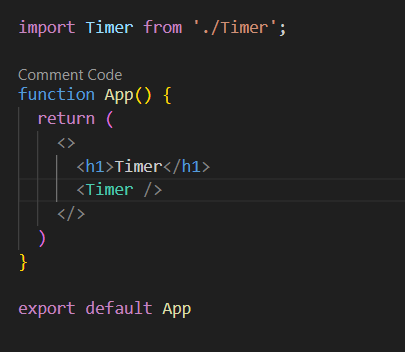
\includegraphics[width=\linewidth]{images/code6.png}
					%\caption{Résultat}
					\label{fig:image2}
				\end{minipage}
			\end{figure}
			\centering
			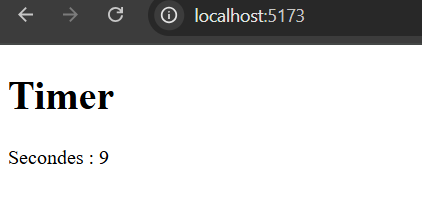
\includegraphics[width=0.4\textwidth]{images/resultat3.png}
		
		\end{exampleblock}
	\end{frame}
	
	
	\section{Bonnes pratiques}
	\begin{frame}{Bonnes pratiques}
		\begin{itemize}
			\item \textbf{Composants purs} : Évitez les effets secondaires dans les composants.
			\item \textbf{État local} : Utilisez l'état local uniquement lorsque nécessaire.
			\item \textbf{Modularité} : Divisez l'application en petits composants réutilisables.
		\end{itemize}
	\end{frame}
	
	\section{Outils pour travailler avec React}
	\begin{frame}{Outils pour travailler avec React}
		\begin{itemize}
			\item \textbf{Create React App} : Outil pour créer rapidement des applications React.
			\item \textbf{React DevTools} : Extension de navigateur pour déboguer les applications React.
			\item \textbf{Redux} : Bibliothèque pour la gestion de l'état global.
		\end{itemize}
	\end{frame}
	
	
	\section{Exemple d'application React}
	\begin{frame}{Exemple d'application React}
		\begin{exampleblock}{Application simple de liste de tâches}
			
			\begin{figure}[h] % "h" pour placer les images ici
				\centering
				\begin{minipage}{0.67\textwidth}
					\centering
					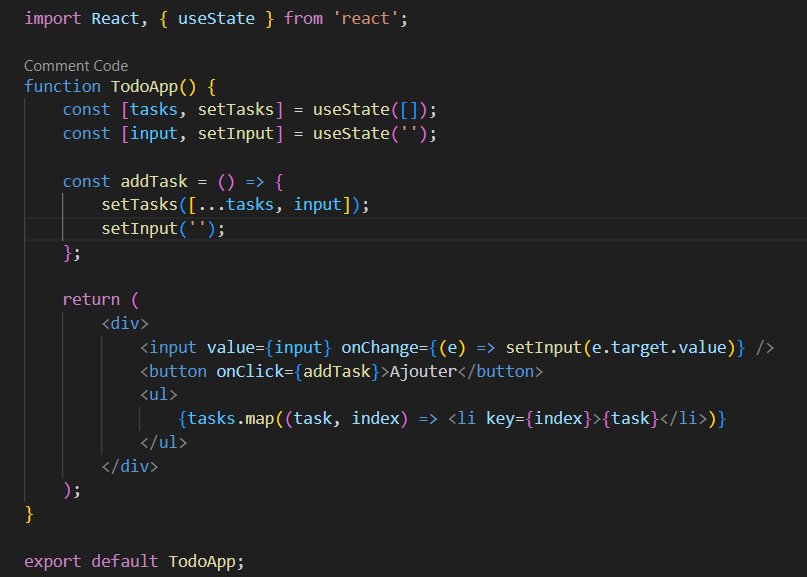
\includegraphics[width=\linewidth]{images/code7.png}
					%\caption{Code}
					\label{fig:image1}
				\end{minipage}
				\hfill % Espace flexible entre les images
				\begin{minipage}{0.29\textwidth}
					\centering
					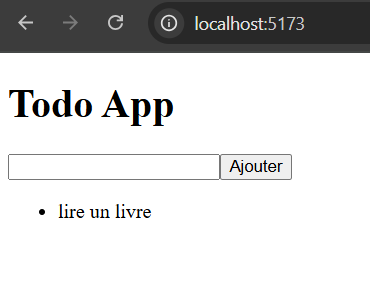
\includegraphics[width=\linewidth]{images/resultat4.png}
					%\caption{Résultat}
					\label{fig:image2}
				\end{minipage}
			\end{figure}
			
			
		\end{exampleblock}
	\end{frame}
	
	\section{Défis de React}
	\begin{frame}{Défis de React}
		\begin{itemize}
			\item \textbf{Courbe d'apprentissage} : React peut être complexe pour les débutants.
			\item \textbf{Gestion de l'état} : La gestion de l'état peut devenir complexe dans les grandes applications.
			\item \textbf{Performances} : Optimisation nécessaire pour les applications très interactives.
		\end{itemize}
	\end{frame}
	
	\section{Pourquoi c'est important ?}
	\begin{frame}{Pourquoi c'est important ?}
		\begin{itemize}
			\item React est largement utilisé dans l'industrie pour construire des interfaces utilisateur modernes.
			\item Il permet de créer des applications web performantes et maintenables.
			\item Comprendre React est essentiel pour les développeurs front-end.
		\end{itemize}
	\end{frame}
	
	
	\begin{frame}{Résumé}
		\textbf{React} est une bibliothèque puissante pour construire des interfaces utilisateur interactives.  
		Explorez, apprenez, et construisez avec React !
	\end{frame}
	

	
\end{document}
